% texto ou documento elaborado pelo autor, a fim de complementar sua argumentação, sem prejuízo da unidade nuclear do trabalho,

% ---
% Inicia os apêndices
% ---
%\apendices
%\partapendices

\begin{apendicesenv}
\partapendices

	% Imprime uma página indicando o início dos apêndices
	\chapter{Circuito Completo}
	\label{Anx1}
		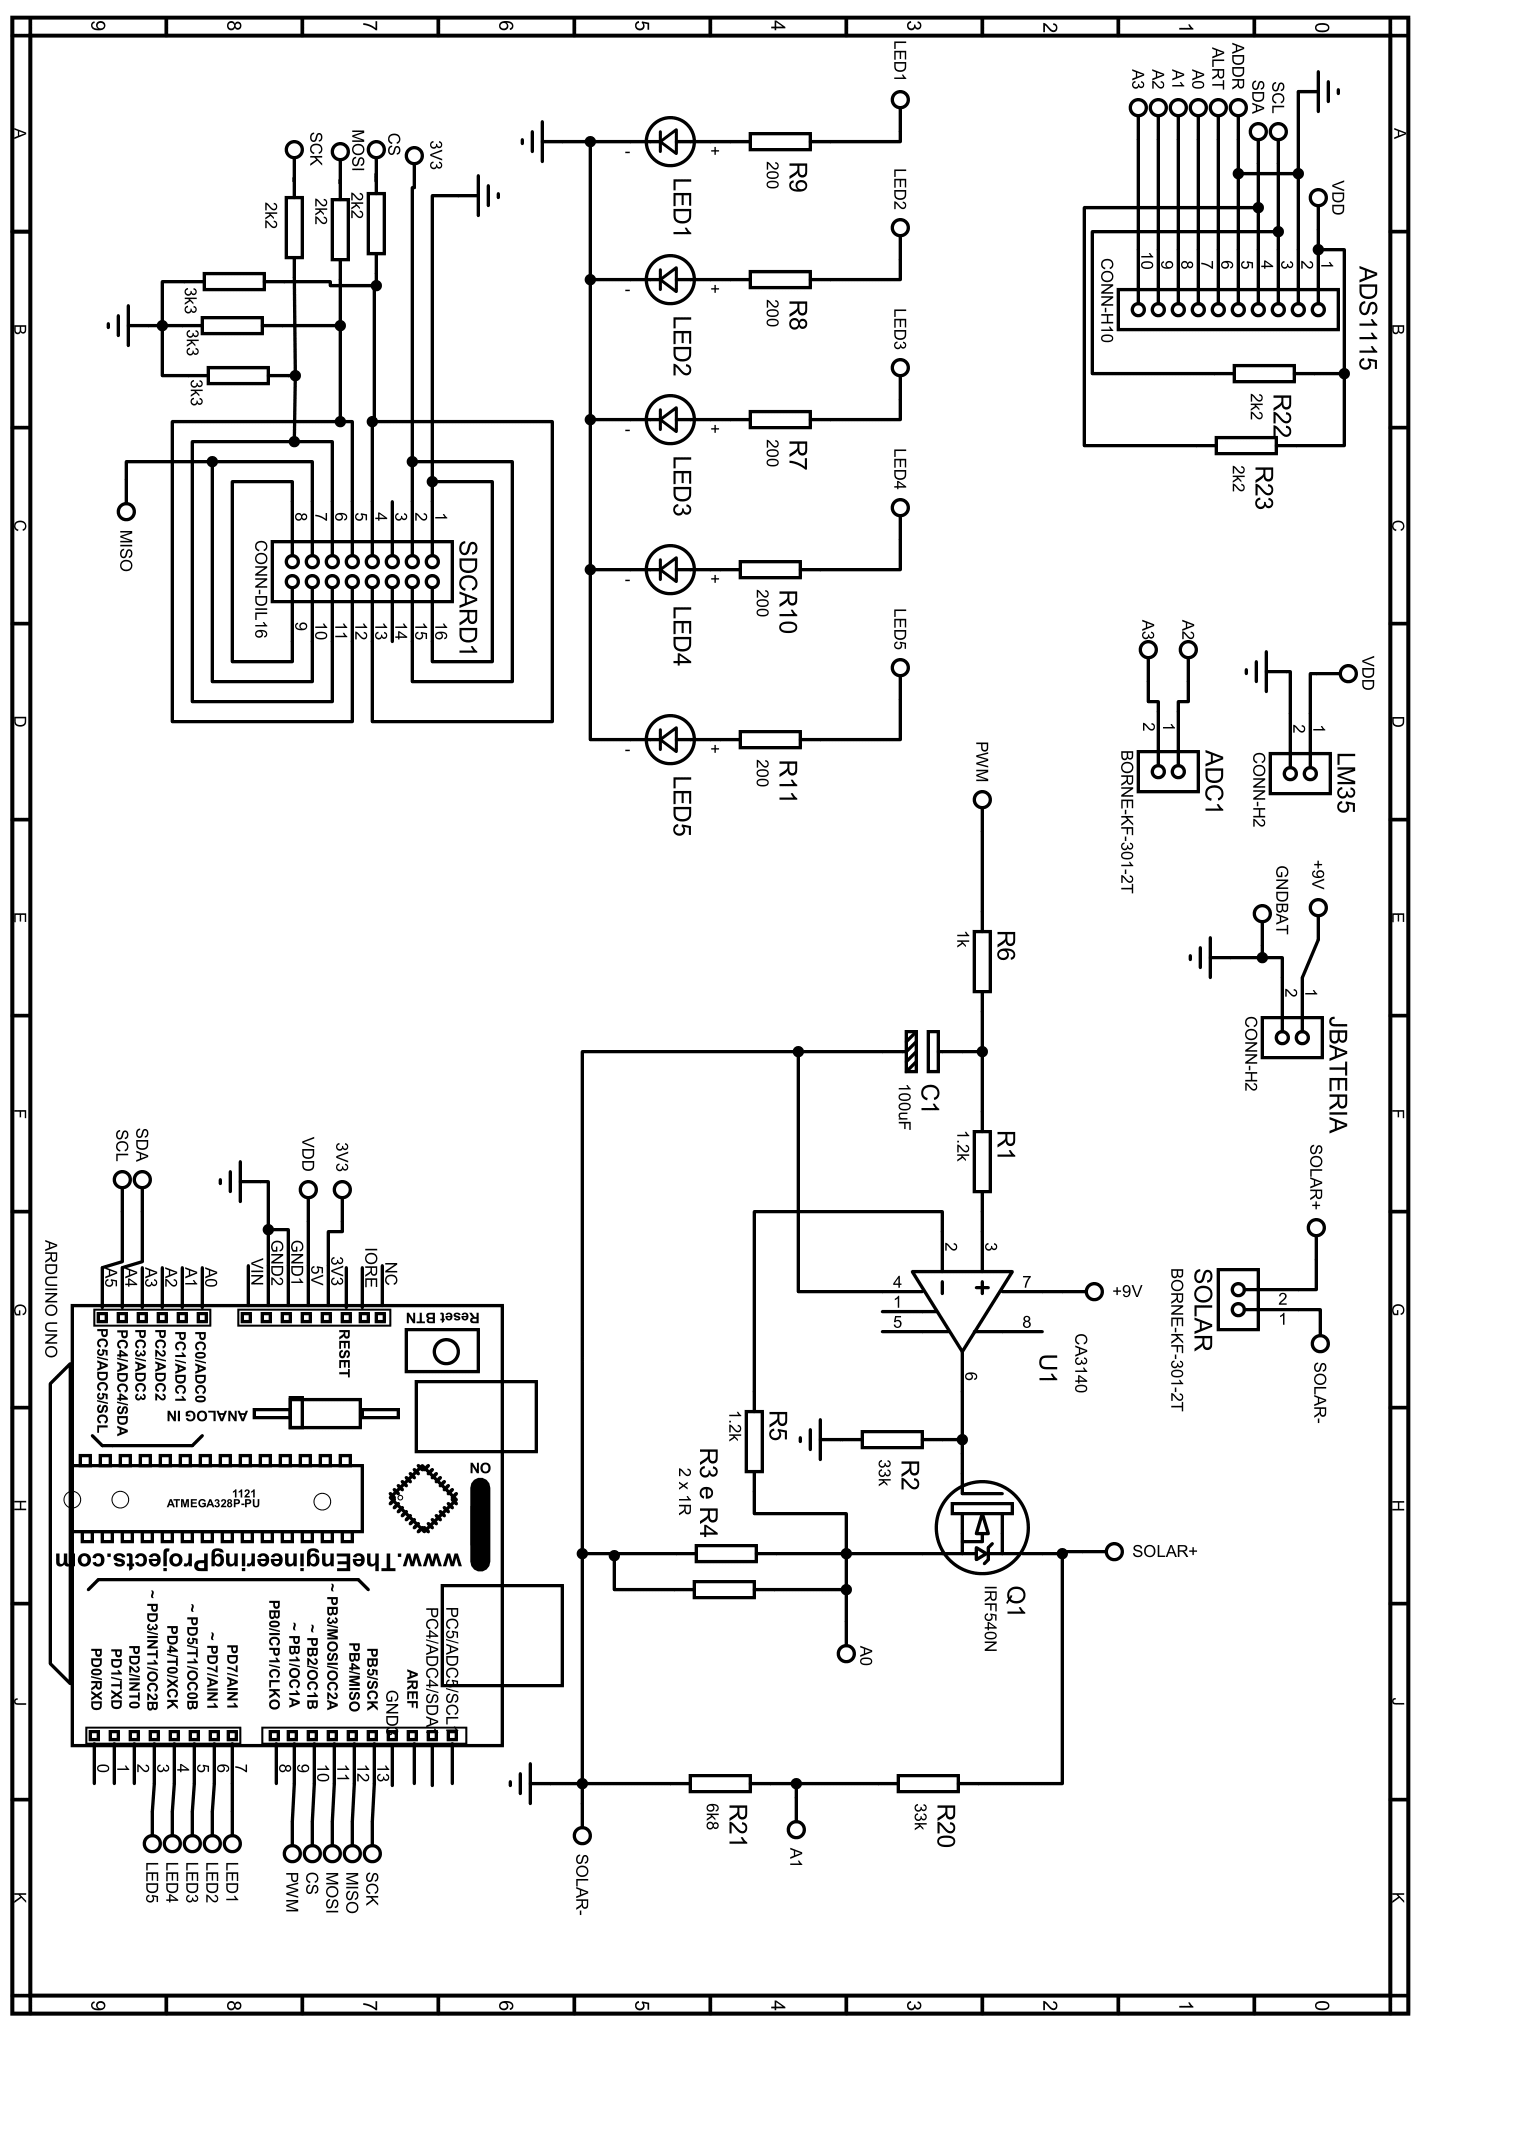
\includegraphics[scale=0.4]{PDFs/AllComponents-rotated-1.png}
	% ----------------------------------------------------------
	\chapter{Título do Apêndice B}
	% ----------------------------------------------------------
	Tabela com o valor gasto para desenvolver um traçador de curva IV.
		\FloatBarrier
		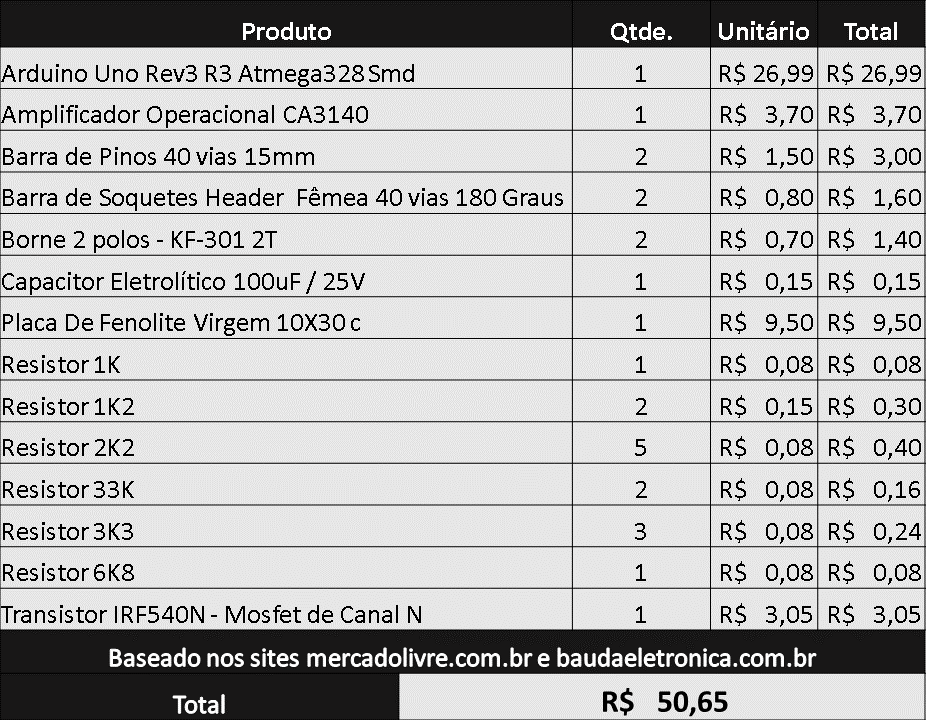
\includegraphics[scale=0.6]{PDFs/values.png}			\FloatBarrier
\end{apendicesenv}
% ---